% Transcribed from blueprint/src/parts/02-line.tex.
\section{The line and its grids}
\label{sec:line-theory}

Images live in the plane, and Section~\ref{ch:price} builds an exact pyramid on the grid
$h\ZZ^d$. Its mask, the frame mask, is a product of masks on the line, one sampled Laplace mask
along each coordinate axis. This section supplies that mask. It computes the mask's \Levy{} measure,
and it shows that the mask is applied by one forward and one backward recursion.

The line is also where the criterion for an exact pyramid, in the sense of the introduction, can be
read in the weights of a mask. Section~\ref{ch:price} proves the criterion in every dimension, and
its case $d = 1$ is stated here. A symmetric probability mask other than $\delta_0$ on a grid of the line has an
exact pyramid exactly when it is infinitely divisible with a logarithmic moment. The families through
such a pyramid lie in stratum~2 and never in stratum~3.

The line is the case $d = 1$ of Section~\ref{ch:pyramid}, and this section uses that section's
results throughout. The line also has axioms of its own, stated for operators $\Phi_{s,t}$ on
$L^1(\RR)$ as (A1)--(A8) and (ND) of Definition~\ref{def:cascade-measurement-family}. Of these, the
covariance axiom (A8) requires covariance under every dilation. A pyramid needs it only at the
dilations $q^n$, $n \in \ZZ$, which form the closed subgroup $q^{\ZZ}$ of $(0,\infty)$. So this
section requires (A8) at those dilations alone. Read through the kernels, these operator axioms are
those of Section~\ref{ch:pyramid} at $d = 1$, and the first subsection proves it. The three
subsections take these points in turn.
\begin{itemize}
\item Section~\ref{subsec:line-strata} reads the operator axioms through their kernels, so that the
statements of Section~\ref{ch:pyramid} hold at $d = 1$. It then places the families of the line
among the three strata.
\item Section~\ref{subsec:grid-pyramids-line} says which masks on a grid have an exact pyramid, and
in which stratum the families through such a pyramid lie.
\item Section~\ref{subsec:sampled-laplace} computes with the sampled Laplace kernels on the grid. It
compares the \Matern{} pyramid, computed by recursion and decimation, with the samples of its
steps.
\end{itemize}
The rest of the theory on the line is in the supplement.

\subsection{The three strata}
\label{subsec:line-strata}

Section~\ref{ch:pyramid} speaks of families of laws, and the axioms of the line speak of operators.
This subsection shows that the two describe the same families, so that every statement of
Section~\ref{ch:pyramid} applies on the line. It then describes the strata in the line's \Levy{}
coordinates, names the knots, and ends with the pyramid principle, which says what covariance means
for sampled kernels.

A statement in $\RR^d$ is read at $d = 1$ through the identification $x \mapsto xe_1$ of $\RR$ with
$\RR^1$. This identification preserves transforms, convolution and dilations. It also preserves
symmetry, infinite divisibility, lattices, the absolute value and Lebesgue measure.

The first definition fixes the operator families of a pyramid on the line. They satisfy (A1)--(A7)
and (ND), and (A8) is required of them at the dilations in $q^{\ZZ}$ only.

% shared with blueprint def:q-covariant-line
\begin{definition}[families on the line covariant under one ratio]
\label{def:q-covariant-line}

Let $q > 1$. A family $(\Phi_{s,t})_{0 \le s \le t}$ of linear operators on $L^1(\RR)$ is
\emph{$q^{\ZZ}$-covariant} if it satisfies (A1)--(A7) and (ND) of
Definition~\ref{def:cascade-measurement-family}, and (A8) required at the dilations in $q^{\ZZ}$:
there are increasing bijections $S_\lambda$ of $[0,\infty)$, $\lambda \in q^{\ZZ}$, with
$\mathcal{D}_\lambda\Phi_{s,t} = \Phi_{S_\lambda s, S_\lambda t}\mathcal{D}_\lambda$ for all
$s \le t$. This condition is written (A8$|q^{\ZZ}$). The family is in the \emph{canonical
discrete gauge} if $S_qt = qt$ for all $t$. It is \emph{fully covariant} if it satisfies
(A1)--(A8) and (ND).
\end{definition}

The next lemma passes between operators and their kernels. Its last sentence is what the rest of the
section uses: a $q^{\ZZ}$-covariant family is, through its kernels, a symmetric $q$-covariant family
in dimension $1$ in the sense of Section~\ref{ch:pyramid}.

% shared with blueprint lem:line-axioms-kernels
\begin{lemma}[the axioms on the line, read on the kernels]
\label{lem:line-axioms-kernels}

Let $(\Phi_{s,t})_{0 \le s \le t}$ be linear operators on $L^1(\RR)$.
\begin{enumerate}
\item If they satisfy (A1)--(A7), then $\Phi_{s,t}f = \mu_{s,t} * f$ for a unique family of
symmetric probability measures $\mu_{s,t}$ on $\RR$, the \emph{kernels}. These satisfy (I1) and
(I2), and (ND) holds if and only if $\mu_{s,t} \ne \delta_0$ for $s < t$. So the kernels of a
family with (A1)--(A7) and (ND) are a symmetric family in dimension $1$
(Definition~\ref{def:family-dimension-d}).
\item Conversely, if symmetric probability measures $\mu_{s,t}$ on $\RR$ satisfy (I1) and (I2),
the operators $\Phi_{s,t}f := \mu_{s,t} * f$ satisfy (A1)--(A7), and they satisfy (ND) if and
only if $\mu_{s,t} \ne \delta_0$ for $s < t$. In particular a symmetric family in dimension $1$
gives a family with (A1)--(A7) and (ND).
\item Let $\lambda > 0$ and let $S$ be an increasing bijection of $[0,\infty)$. Then
$\mathcal{D}_\lambda\Phi_{s,t} = \Phi_{Ss,St}\mathcal{D}_\lambda$ for all $s \le t$ if and only
if $T_\lambda\mu_{s,t} = \mu_{Ss,St}$ for all $s \le t$. So (A8) at the dilation $\lambda$ is
$\lambda$-covariance of the kernels, with the same bijection.
\end{enumerate}
So the $q^{\ZZ}$-covariant families (Definition~\ref{def:q-covariant-line}) are, read through their
kernels, the symmetric $q$-covariant families in dimension $1$, with the same bijections.
\end{lemma}

\begin{proof}
Write $g(x) := (2\pi)^{-1/2}e^{-x^2/2}$, whose transform $\widehat g(\omega) = e^{-\omega^2/2}$
has no zero. For a finite measure $\mu$ the transform of $\mu * g$ is $\widehat\mu\,\widehat g$,
so the operator $f \mapsto \mu * f$ determines $\widehat\mu$, hence $\mu$.

(1) By Theorem~\ref{thm:cited-A1}, under (A1), (A2), (A4) and (A5) each
$\Phi_{s,t}$ is the convolution with a unique probability measure $\mu_{s,t}$, which is
symmetric under (A3). (A6) reads $\delta_0 * f = \mu_{t,t} * f$ and
$(\mu_{s,t} * \mu_{r,s}) * f = \mu_{r,t} * f$ for every $f \in L^1$, by the associativity of
convolution. By the remark above this is $\mu_{t,t} = \delta_0$ and
$\mu_{r,t} = \mu_{s,t} * \mu_{r,s}$, which is (I1). For (I2) let $(s_n,t_n) \to (s,t)$ in
$\{0 \le s \le t\}$. Since the transform of an integrable function is bounded by its $L^1$ norm,
\[
  \bigl|\widehat\mu_{s_n,t_n}(\omega) - \widehat\mu_{s,t}(\omega)\bigr|\,\widehat g(\omega)
  \le \bigl\|\mu_{s_n,t_n} * g - \mu_{s,t} * g\bigr\|_1 ,
\]
and the right side tends to $0$ by (A7). Since $\widehat g(\omega) > 0$, this is (I2). Finally
$\Phi_{s,t} = \mathrm{Id}$ if and only if $\mu_{s,t} = \delta_0$, by the remark above.

(2) The converse half of Theorem~\ref{thm:cited-A1} gives (A1)--(A5). (A6) is (I1) and the
associativity of convolution, and $\Phi_{s,t} \ne \mathrm{Id}$ if and only if
$\mu_{s,t} \ne \delta_0$, by the remark above. For (A7) write $\tau_yf := f(\cdot - y)$ and
$\Theta_f(y) := \|\tau_yf - f\|_1$, a bounded continuous function with $\Theta_f(0) = 0$, by the
continuity of translation in $L^1$. For a probability $\nu$, $\nu * f - f$ is the
$\nu$-average of $\tau_yf - f$, so $\|\nu * f - f\|_1 \le \int\Theta_f\,d\nu$. Let
$(s_n,t_n) \to (s,t)$ and move one endpoint at a time,
through $(s_n, t)$ when $s_n \le t$, and through $(s, t_n)$ otherwise, where
$s \le t < s_n \le t_n$. By (I1),
$\mu_{s,t} * f - \mu_{s',t} * f = \mu_{s'',t} * (\mu_{u,v} * f - f)$ up to sign, with
$u = \min(s, s')$, $v = \max(s, s')$ and $s''$ the larger of the two, so
$\|\mu_{s,t} * f - \mu_{s',t} * f\|_1 \le \|\mu_{u,v} * f - f\|_1 \le \int\Theta_f\,d\mu_{u,v}$,
convolution with a probability being a contraction of $L^1$. In the same way
$\|\mu_{s,t} * f - \mu_{s,t'} * f\|_1 \le \int\Theta_g\,d\mu_{\min(t,t'),\max(t,t')}$ with $g$ the
convolution of $f$ with the earlier factor, and $\Theta_g \le \Theta_f$ since translation commutes
with convolution. As the two ends of an increment tend to a common limit $c$, its transform tends
to $\widehat\mu_{c,c} = 1$ by (I2), so the increment tends weakly to $\delta_0$ by \Levy's
continuity theorem, and $\int\Theta_f$ against it tends to $\Theta_f(0) = 0$. This gives (A7).

(3) For a probability $\mu$ and $f \in L^1$,
\[
  (T_\lambda\mu) * (\mathcal{D}_\lambda f)(x) = \int\lambda^{-1}f\bigl((x - \lambda y)/\lambda\bigr)\,\mu(dy)
  = \lambda^{-1}(\mu * f)(x/\lambda) = \mathcal{D}_\lambda(\mu * f)(x) .
\]
So $\mathcal{D}_\lambda\Phi_{s,t}f = (T_\lambda\mu_{s,t}) * \mathcal{D}_\lambda f$, while
$\Phi_{Ss,St}\mathcal{D}_\lambda f = \mu_{Ss,St} * \mathcal{D}_\lambda f$. Since
$\mathcal{D}_\lambda$ maps $L^1$ onto $L^1$, the two operators agree for every $f$ if and only if
the convolutions with $T_\lambda\mu_{s,t}$ and with $\mu_{Ss,St}$ agree on all of $L^1$, that is,
by the remark above, if and only if $T_\lambda\mu_{s,t} = \mu_{Ss,St}$.

For the last sentence, by (1)--(3) a family with (A1)--(A7), (ND) and (A8) at every
$\lambda \in q^{\ZZ}$ is, through its kernels, a symmetric family in dimension $1$ that is
$\lambda$-covariant at every $\lambda \in q^{\ZZ}$, with the same bijections, and conversely. In
particular it is $q$-covariant. Conversely a $q$-covariant symmetric family is
$\lambda$-covariant at every $\lambda \in q^{\ZZ}$, since the set of $\lambda$ at which it is
covariant is a group, with $S_{q^n} = S_q^n$ (Lemma~\ref{lem:family-dilations}(1)--(2)):
covariance at $\lambda$ with $S$ and at $\lambda'$ with $S'$ gives covariance at $\lambda\lambda'$
with $S \circ S'$, and at $\lambda^{-1}$ with $S^{-1}$, so $S_q$ iterated $n$ times serves $q^n$,
and its inverse iterated serves $q^{-n}$.

Every step is machine-checked, Theorem~\ref{thm:cited-A1} included.
\end{proof}

The strata of Section~\ref{ch:pyramid} are described by \Levy{} data, and on the line these data
take a simpler form. A symmetric measure on $\RR$ is determined by its image under
$x \mapsto |x|$, its \emph{fold}. So the line's statements carry a symmetric \Levy{} measure as a
measure on $(0,\infty)$, which gives the rate of the jumps of each length. The next definition names
the pair this gives.

% shared with blueprint def:folded-data
\begin{definition}[folded data]
\label{def:folded-data}

For a symmetric infinitely divisible law on $\RR$ with exponent
$\Psi(\omega) = a\omega^2 + \int_{(0,\infty)}(1 - \cos\omega v)\,\varpi(dv)$, the pair
$(a, \varpi)$ is its \emph{folded data}: $a$ is the Gaussian coefficient and $\varpi$ the image
of the \Levy{} measure under $x \mapsto |x|$.
\end{definition}

\paragraph{The strata on the line.} One fact is special to the line. Since
$\Orth(1) = \{\pm1\}$, a symmetric family on the line is isotropic. So through
Lemma~\ref{lem:line-axioms-kernels} the statements of Section~\ref{ch:pyramid} hold on the line at
$d = 1$, those about isotropic families included. The three nested strata of
Section~\ref{sec:pyramid-strata} are among them.

Covariance behaves on the line as in $\RR^d$. The dilations of a family form $\{1\}$, some
$q^{\ZZ}$ or $(0,\infty)$ (Lemma~\ref{lem:family-dilations}(2)). Under covariance at $q$ a
relabelling of the scales gives the canonical discrete gauge $S_qt = qt$
(Lemma~\ref{lem:family-dilations}(4)). Under $q^{\ZZ}$ the gauge is unique only up to the group
$\mathcal{G}_q$ of Lemma~\ref{lem:gauge-group}.

In folded data, covariance and the strata take a concrete form. Write $(a(t), \varpi_t)$ for the
folded data of the kernel $\mu_{0,t}$. The family is $q$-covariant with $S_qt = qt$ if and only if
$a(qt) = q^2a(t)$ and $\varpi_{qt} = T_q\varpi_t$ for all $t > 0$. Every kernel is then
semi-selfdecomposable with span $q$, and the kernels at the scales in $[1, q)$ determine the family
(Lemma~\ref{lem:discrete-covariance-levy}).

Semi-selfdecomposability is meant in the sense of Maejima and Naito [\sscite{maejima1998semi}]
(Definition~\ref{def:self-decomposable}). On the line a symmetric law $\mu$ is
semi-selfdecomposable with span $q > 1$ when
$\widehat\mu(\omega) = \widehat\mu(\omega/q)\,\widehat\varrho_q(\omega)$ for some infinitely
divisible law $\varrho_q$, the residual (Definition~\ref{def:self-decomposable} at $d = 1$). Sato's
criteria for semi-selfdecomposability are recalled in Section~\ref{sec:pyramid-strata}, and folded
data give a short test. For a symmetric law with folded data $(a, \varpi)$ the criterion
$T_q\nu \ge \nu$ of Theorem~\ref{thm:cited-A44} reads $T_q\varpi \ge \varpi$. This holds because
folding commutes with $T_q$ and a symmetric measure is determined by its fold.

Theorem~\ref{thm:lattice-strata} gives the three strata in these coordinates. Its clause (3), read
through Theorem~\ref{thm:cited-A4}, describes stratum~3. A fully covariant family, relabelled by
its gauge, has $a(t) = \alpha t^2$ and $\varpi_t(dv) = k(v/t)\,v^{-1}dv$, with $(\alpha, k)$ the
data of an admissible exponent.

The examples of Section~\ref{sec:pyramid-strata} separate the strata on the line too. At $d = 1$
the uniform law on the sphere of radius $h$ is $\tfrac12(\delta_h + \delta_{-h})$. The family of
Proposition~\ref{prop:stratum-one-example} is then Lindeberg's discrete scale space
[\sscite{lindeberg1990scalespace}], with $\varpi_t = t\,\delta_h$. It is in the first stratum and
not in the second. The family of Proposition~\ref{prop:stratum-two-example} is the
\emph{geometric-jump pyramid}, whose jumps have the lengths $hq^i$, $i \in \ZZ$. It is in the second
stratum and not in the third. With these witnesses
Theorem~\ref{thm:lattice-strata-strict} separates the strata on the line. No kernel $\mu_{0,t}$,
$t > 0$, of a $q^{\ZZ}$-covariant family is carried by a lattice $\xi\ZZ$
(Proposition~\ref{prop:no-lattice-kernel}).

Section~\ref{supp:strata} of the supplement states and proves these statements in the line's own
terms, the operator axioms and the folded data. The counterparts are the following.
\begin{itemize}
\item Lemma~\ref{lem:family-dilations}(2): Lemma~\ref{lem:closed-subgroups}.
\item Lemma~\ref{lem:discrete-covariance-levy}: Lemma~\ref{lem:discrete-covariance-line}.
\item Theorem~\ref{thm:lattice-strata}: Theorem~\ref{thm:lattice-line}.
\item Proposition~\ref{prop:stratum-one-example}: Proposition~\ref{prop:lindeberg-stratum-one}.
\item Proposition~\ref{prop:stratum-two-example}: Proposition~\ref{prop:discrete-gaussian-pyramid}.
\item Theorem~\ref{thm:lattice-strata-strict}: Theorem~\ref{cor:lattice-line-strict}.
\item Proposition~\ref{prop:no-lattice-kernel}: Proposition~\ref{prop:no-lattice-kernel-line}.
\end{itemize}

\paragraph{Knots.} A pyramid stores its levels at the knots, and the grid pyramids below are read
there. The knots, the knot kernels and the ladder of a $q^{\ZZ}$-covariant family in the canonical
discrete gauge are those of its kernels (Lemma~\ref{lem:line-axioms-kernels}), in the sense of
Definition~\ref{def:knots-and-ladder} at $d = 1$. The knots are the scales $q^n$, $n \in \ZZ$, the
ends of the annuli $[q^n, q^{n+1}]$. With the exponents $\Psi_t := -\log\widehat\mu_{0,t}$ of
Lemma~\ref{lem:family-structure}, the knot kernels $\mu_{0,q^n}$ have
$\Psi_{q^n} = \Psi_1(q^n\,\cdot)$ (Lemma~\ref{lem:discrete-covariance-levy}). So they are the
dilates of the one knot kernel $\mu_{0,1}$. Which scale is called $1$ is a choice of gauge
(Lemma~\ref{lem:gauge-group}), and the statements below fix it.

\paragraph{The pyramid principle.} An implemented pyramid works with arrays on grids, so the next
question is what covariance says about them. A step $\mu_{s,t}$ with $s > 0$, unlike a kernel, can
be a lattice law, and a grid pyramid applies such steps. The kernels themselves are carried by no
lattice (Proposition~\ref{prop:no-lattice-kernel}). Where they have continuous densities, an
implemented pyramid can sample them on grids. For an integer $q$ the knot kernels of an exact grid
pyramid have none: they are singular (Proposition~\ref{prop:grid-pyramid-singular-kernels}).
What covariance says about the samples, where they exist, is the pyramid principle of
Section~\ref{ch:pyramid} at $d = 1$, Proposition~\ref{prop:no-lattice-kernel-line}(2). In the canonical discrete gauge, if $\mu_{0,t}$
has a continuous density $\phi_t$ for some $t > 0$, then $q^n\phi_{q^nt}(q^nhm) = \phi_t(hm)$ for
all $n \in \ZZ$, $h > 0$ and $m \in \ZZ$. Sampled at the scale $q^nt$ on the grid $q^nh\ZZ$, the
kernel is the same array at every level, up to the factor $q^n$.
Figure~\ref{fig:pyramid-schematic} shows the knots, the grids and the one mask applied at every
level.

\subsection{Grid pyramids: which masks have a pyramid, and in which stratum}
\label{subsec:grid-pyramids-line}

A pyramid of the literature is given by its mask, an array of positive weights on a grid. The
question for such a pyramid is whether some family of the axioms has the mask, dilated to each
level, as its ladder. Section~\ref{ch:pyramid} answered it for laws in $\RR^d$, lattice laws
included. A symmetric law other than $\delta_0$ is the octave step $\mu_{1,q}$ of a symmetric
$q$-covariant family in the canonical discrete gauge exactly when it is infinitely divisible with a
logarithmic moment (Proposition~\ref{prop:ladder-knot-kernel}). This subsection reads that answer
for masks on a grid of the line, in the operator axioms. The criterion of the next proposition
rests on Proposition~\ref{prop:ladder-knot-kernel} at $d = 1$. The subsection also says in which
stratum the families through such a pyramid lie.

The finite masks of the classical pyramids are already excluded. A law of bounded support other
than a point mass is a step of no family with (I1) and (I2)
(Proposition~\ref{prop:no-bounded-step}). But a mask need not be finite to be implementable. The
sampled Laplace mask has infinitely many nonzero weights, and it is applied by one forward and one
backward recursion (Proposition~\ref{prop:recursion-helmholtz}(2)). So the criterion has to be read
on infinite masks, where it becomes a condition on the weights.

The stratum needs an argument of its own. In the continuum, for steps with a rational transform,
\prog{V-cone v0.1}{Prop.~7.5(2), p.~65} (Theorem~\ref{thm:cited-A20}) decides whether the covariant
interpolant of the step is admissible, the exponent of a fully covariant family. Its criterion is a
condition on the \Levy{} profile: the sum of the dilates of the profile must have a nonincreasing
version. The \Levy{} measure of a lattice mask is atomic, so it has no profile, and this criterion
does not apply to it. Clause (3) of the next proposition settles the question on the lattice
instead. Throughout, $h > 0$ is the grid spacing and $\vartheta = h\omega$ the grid frequency.

% shared with blueprint def:grid-pyramid-line
\begin{definition}[the grid pyramid of a mask]
\label{def:grid-pyramid-line}

Let $q > 1$ and $h > 0$, and let $w \ne \delta_0$ be a symmetric probability law on $h\ZZ$, the
\emph{mask}. The \emph{grid pyramid} of $(w, q)$ is the ladder $\mu_{q^n,q^{n+1}} := T_{q^n}w$,
$n \in \ZZ$, read in the canonical discrete gauge $S_qt = qt$, so that its knots are the scales
$q^n$: the same array, applied on the grid $q^nh\ZZ$ at every level. It is
\emph{exact} if some $q^{\ZZ}$-covariant family in the canonical discrete gauge has these
steps, through its kernels (Lemma~\ref{lem:line-axioms-kernels}), and \emph{exact in the third stratum} if
some such family is fully covariant.
\end{definition}

The definition is the pyramid principle read on the steps rather than on the kernels. Only one step
has to be checked. Under (A8$|q^{\ZZ}$) with $S_qt = qt$ the one requirement $\mu_{1,q} = w$
already forces the ladder, since covariance at $q^n$ gives $T_{q^n}\mu_{1,q} = \mu_{q^n,q^{n+1}}$
(Lemma~\ref{lem:line-axioms-kernels}(3)). So either notion is a condition on one step.

Exactness here is the sense of the introduction. On a grid the word \emph{exact} has three senses,
fixed in Definition~\ref{def:exact-senses} of Section~\ref{ch:price}, and this section uses all
three. A fourth phrase stands apart.
\begin{itemize}
\item A grid computation is exact in sense (i) when the arrays it produces, in exact arithmetic,
equal the kernels they stand for. A continuum kernel stands for its renormalized samples.
\item The subsample of a member of a grid family is exact in sense (ii) when, renormalized to mass
one, it is a member of the same family on the coarser grid.
\item A grid pyramid is exact in sense (iii) when a family continuous in scale and covariant under
$q$ carries its ladder. On the line this is the exactness of the definition above.
\item An \emph{exact cascade on the grid} is a family on one grid whose increments are again grid
kernels. The phrase names none of the three senses.
\end{itemize}
Exactness in the third stratum requires in addition that the carrying family be fully covariant.
Definition~\ref{def:exact-grid-pyramid} states the notion in $\RR^d$, on laws, and this definition
is its operator form on the line. The two agree at $d = 1$
(Proposition~\ref{prop:line-and-arrays}(1)).

The next proposition answers the question of this subsection. A mask has an exact grid pyramid
exactly when it is infinitely divisible and has a logarithmic moment,
$\int\log_+|x|\,w(dx) < \infty$. Since $\log_+x \le x^p/(pe)$ for $x \ge 0$ and $p > 0$, every
mask with a finite moment of some positive order has it. Every family through an exact grid pyramid then lies in stratum~2 and not in stratum~3. Clause (1)
says which masks are infinitely divisible, and clause (4) applies the criterion to the sampled
Laplace mask and to the classical finite masks. For laws the sufficiency is the theorem of Maejima
and Ueda [\sscite{maejima2009stochastic}, Thm.~3.3, p.~353]. The necessity of infinite divisibility
comes from continuity in scale (Lemma~\ref{lem:steps-infinitely-divisible}).

Clause (1) also places the exact masks against Burt's equal contribution. An exact mask has a
positive transform. For an integer ratio $r$, equal contribution requires
$\sum_iw(h(j + ir)) = 1/r$ for every $j$ [\sscite{burt1981fast}, (C4), p.~23], which Burt and
Adelson state for $r = 2$ [\sscite{burt1983laplacian}, p.~533]. In transforms it requires
$\widehat w$ to vanish at the frequencies $2\pi k/(rh)$, $0 < k < r$. So no exact mask has equal
contribution at an integer ratio. Burt motivates the condition by the equal weight of every sample
under reduction and by the convergence of the equivalent kernels [\sscite{burt1981fast}, p.~24].

% shared with blueprint prop:grid-pyramids-infinitely-divisible
\begin{proposition}[grid pyramids and infinitely divisible masks]
\label{prop:grid-pyramids-infinitely-divisible}

Let $q > 1$, $h > 0$, and let $w \ne \delta_0$ be a symmetric probability law on $h\ZZ$.
\begin{enumerate}
\item \emph{(Lattice carrier.)} The mask $w$ is infinitely divisible if and only if it is compound
Poisson,
\[
  \widehat w(\omega) = \exp\Bigl(-\int_{(0,\infty)}(1 - \cos\omega v)\,\varpi_w(dv)\Bigr),
\]
with a finite measure $\varpi_w \ne 0$ carried by $h\ZZ_{>0}$, its folded \Levy{} measure. Then
$\widehat w > 0$ everywhere and the support of $w$ is unbounded. So a mask of bounded support is
not infinitely divisible.
\item \emph{(Criterion, and the covariant kernel.)} The grid pyramid of $(w, q)$ is exact if
and only if
\begin{equation}
\label{eq:grid-pyramid-criterion}
  w \text{ is infinitely divisible and } \int_{(0,\infty)}\log_+v\;\varpi_w(dv) < \infty ,
\end{equation}
equivalently if and only if $w$ is infinitely divisible and $\int\log_+|x|\,w(dx) < \infty$. Its
knot kernel is then unique: every family carrying the ladder has $a(1) = 0$ and
\begin{equation}
\label{eq:grid-pyramid-knot-kernel}
  \varpi_1 = \sum_{m \ge 1}T_{q^{-m}}\varpi_w, \qquad
  \widehat\mu_{0,1}(\omega) = \prod_{m \ge 1}\widehat w(q^{-m}\omega),
\end{equation}
the product being the limit of the transforms of $T_{q^{-1}}w * \dots * T_{q^{-M}}w$ as
$M \to \infty$. The measure $\varpi_1$ is carried by the union of the sets $q^{-m}h\ZZ_{>0}$,
$m \ge 1$, and by no lattice $\xi\ZZ$. When $w$ is infinitely divisible and
$\int\log_+v\;\varpi_w(dv) = \infty$, the partial products
have no limit that is a characteristic function, and they tend to $0$ at almost every $\omega$,
though not in general at every $\omega \ne 0$ (at $q = 2$, by
Proposition~\ref{prop:ladder-not-every-frequency}): there is no kernel. The families carrying the ladder
are not unique. One of them is the \emph{uniform coupling}, with $a(t) = 0$ and
$\varpi_t = \varpi_1 + (\log_qt)\,\varpi_w$ for $t \in [1,q]$, each atom of the mask switched on
linearly in $\log t$ across the octave.
\item \emph{(No grid pyramid is exact in the third stratum.)} For no $q > 1$, $h > 0$ and mask $w$ is the
grid pyramid of $(w, q)$ exact in the third stratum. More generally, a symmetric law $\varrho \ne \delta_0$
carried by a lattice $\xi\ZZ$, $\xi > 0$, is a step $\mu_{s,t}$ of no fully covariant family. So
every family carrying an exact grid pyramid lies in the second stratum of
Theorem~\ref{thm:lattice-line} and not in the third: the pyramid has a covariant kernel, unique at
the knots, and no fully covariant family interpolates its levels.
\item \emph{(Instances.)} For $0 < a < 1$ the \emph{sampled Laplace mask}
$\lambda^{\mathrm{L}}_a$, the law on $h\ZZ$ with $\lambda^{\mathrm{L}}_a(\{hn\}) =
\tfrac{1-a}{1+a}a^{|n|}$, is infinitely divisible, with all moments finite. So the
\emph{geometric pyramid}, the grid pyramid of $(\lambda^{\mathrm{L}}_a, q)$, is exact for
every $q > 1$, with the unique knot kernel
\begin{equation}
\label{eq:geometric-pyramid-knot-kernel}
  \widehat\mu_{0,1}(\omega) = \prod_{m \ge 1}\Bigl[1 + 2\varsigma\bigl(1 - \cos(q^{-m}h\omega)\bigr)\Bigr]^{-1},
  \qquad \varsigma := \frac{a}{(1-a)^2},
\end{equation}
and by (3) it lies in no stratum above the second.
No mask of bounded support has an exact grid pyramid. Among these masks are two families of odd
length: the binomial masks with the weights $4^{-k}\binom{2k}{k+n}$ at $hn$, $|n| \le k$,
$k \ge 1$, which are the refinement masks of the B-splines of odd degree $2k - 1$ and include
$\tfrac1{16}[1,4,6,4,1]$ at $k = 2$, and the sampled B-spline masks, the values $\beta(n)$, $n \in \ZZ$, of a B-spline $\beta$
of degree at least $2$ with unit knot spacing, centred at $0$, placed at $hn$ and renormalized to unit
mass.
\end{enumerate}
\end{proposition}

\begin{proof}
A measure $\varpi$ on $(0,\infty)$ has the symmetrization $\varpi_s$, the symmetric measure on
$\RR$ that puts half of $\varpi$ on each side of $0$. Then $\varpi_s(B) = \tfrac12\varpi(B)$ for
$B \subseteq (0,\infty)$, so a measure on $(0,\infty)$ is determined by its symmetrization, and
symmetrization commutes with sums and with dilations. Since $\cos$ is even,
$\int(1 - \cos\omega x)\,\varpi_s(dx) = \int_{(0,\infty)}(1 - \cos\omega v)\,\varpi(dv)$. So
$(a, \varpi)$ is a folded pair of the exponent of a law $m$ on $\RR$ if and only if $m$ has the
data $(a, \varpi_s)$.

(1) Let $w$ be infinitely divisible, with folded data $(a, \varpi_w)$
(Lemma~\ref{lem:line-exponent-data}(1)). Then $w$, carried by the lattice $h\ZZ$, has the data
$(a, (\varpi_w)_s)$, the generating triplet $(2a, (\varpi_w)_s, 0)$ in Sato's normalization
(Lemma~\ref{lem:symmetric-levy-khintchine}). By
Lemma~\ref{lem:lattice-infinitely-divisible} at $d = 1$, $2a = 0$, and $(\varpi_w)_s$ is finite and
carried by $h\ZZ \setminus \{0\}$. Hence $\varpi_w = 2(\varpi_w)_s$ on $(0,\infty)$ is finite and
carried by $h\ZZ_{>0}$. So $-\log\widehat w(\omega) = \int(1 - \cos\omega v)\,\varpi_w(dv)$, the
display, and $\widehat w > 0$. And $\varpi_w \ne 0$, since otherwise $w = \delta_0$.
Conversely, let $\widehat w$ have this form with $\varpi_w$ finite. Put
$|\varpi_w| := \varpi_w\bigl((0,\infty)\bigr)$ and let $\sigma$ be the symmetric law
$|\varpi_w|^{-1}(\varpi_w)_s$ on $\RR$. Then $\widehat w = e^{|\varpi_w|(\widehat\sigma - 1)}$
is the transform of the compound Poisson law
$\sum_{k \ge 0}e^{-|\varpi_w|}\tfrac{|\varpi_w|^k}{k!}\sigma^{*k}$, and the $n$-th power of
$e^{(|\varpi_w|/n)(\widehat\sigma - 1)}$, a transform of the same kind, for every $n$. So $w$ is
infinitely divisible. The mask, symmetric and other than $\delta_0$, is not a point mass. So by
Proposition~\ref{prop:no-bounded-step} at $d = 1$ an infinitely divisible mask has unbounded
support, and a mask of bounded support is not infinitely divisible.

(2) Suppose the grid pyramid is exact, carried by a $q^{\ZZ}$-covariant family in the
canonical discrete gauge. By Lemma~\ref{lem:line-axioms-kernels} and
Lemma~\ref{lem:discrete-covariance-line} its kernels are a symmetric family in dimension $1$,
$q$-covariant with $S_qt = qt$ and the step $\mu_{1,q} = w$. Its step $w$ is infinitely divisible
(Lemma~\ref{lem:family-structure}), so by (1) $w$ has the data $(0, (\varpi_w)_s)$.
Proposition~\ref{prop:ladder-knot-kernel}(1) at $d = 1$ gives
$\int\log_+|x|\,(\varpi_w)_s(dx) < \infty$, which is $\int\log_+v\;\varpi_w(dv) < \infty$. It
also gives the product formula, $A_1 = A_w/(q^2 - 1) = 0$ and
$\nu_1 = \nu^* = \sum_{m \ge 1}D_{q^{-m}}(\varpi_w)_s$, the symmetrization of
$\varpi_1 = \sum_{m \ge 1}T_{q^{-m}}\varpi_w$. By the first paragraph and the uniqueness of the
folded data (Lemma~\ref{lem:line-exponent-data}(1)), $a(1) = 0$ and $\mu_{0,1}$ has the folded
measure $\varpi_1$. These depend on $w$ only, so the knot kernel is unique. The partial products
are the transforms of the partial convolutions, by $\widehat{T_c m}(\omega) = \widehat m(c\omega)$
and the convolution theorem.

Conversely, let $w$ be infinitely divisible with the moment. By (1), $\varpi_w$ is finite and
nonzero, and $w$ is a symmetric infinitely divisible law on $\RR$, other than $\delta_0$, with the
data $(0, (\varpi_w)_s)$ and $\int\log_+|x|\,(\varpi_w)_s(dx) = \int\log_+v\;\varpi_w(dv) < \infty$.
Proposition~\ref{prop:ladder-knot-kernel}(2) at $d = 1$ gives a symmetric $q$-covariant family in
dimension $1$ with $S_qt = qt$ and the step $\mu_{1,q} = w$. By
Lemma~\ref{lem:line-axioms-kernels}(2) its laws are the kernels of a family with (A1)--(A7) and
(ND), which by Lemma~\ref{lem:discrete-covariance-line} satisfies (A8$|q^{\ZZ}$) in the canonical
discrete gauge. Covariance at $q$, iterated and inverted, gives
$\mu_{q^ns,q^nt} = T_{q^n}\mu_{s,t}$ for every $n \in \ZZ$, so
$\mu_{q^n,q^{n+1}} = T_{q^n}w$: the pyramid is exact. Proposition~\ref{prop:ladder-knot-kernel}(2)
at $d = 1$, applied to $w$, gives two families with the ladder of $w$ that differ at some pair
of scales. The same clause makes the moment of $(\varpi_w)_s$ equivalent to
$\int\log_+|x|\,w(dx) < \infty$.

The measure $\varpi_w \ne 0$ is carried by the countable set $h\ZZ_{>0}$, so it has an atom
$v_0 \in h\ZZ_{>0}$, and $T_{q^{-m}}\varpi_w$ is carried by $q^{-m}h\ZZ_{>0}$. So $\varpi_1$ is
carried by the union of these sets, with the atoms $q^{-m}v_0 \to 0$. A measure carried by $\xi\ZZ$
has no atom in $(0, \xi)$, so $\varpi_1$ is carried by no lattice.

Let $w$ be infinitely divisible without the moment. Then
Proposition~\ref{prop:ladder-knot-kernel}(3) at $d = 1$, applied to $w$, says that the partial
products have no limit that is a characteristic function, and that they tend to $0$ at almost
every $\omega$. No family
carries the ladder, as one would force the moment by the ``only if'' direction above. The partial
products need not tend to $0$ at every $\omega \ne 0$. Take $q = 2$, let $\varrho$ be the law on
$\ZZ$ of Proposition~\ref{prop:ladder-not-every-frequency}, and put
$w := T_h\varrho$. Its transform $\widehat w(\omega) = \widehat\varrho(h\omega)$ has the form of
(1) with the finite measure $\varpi_w = \sum_{j \ge 1}j^{-2}\delta_{h2^j} \ne 0$, so $w$ is
infinitely divisible, symmetric, other than $\delta_0$ and carried by $h\ZZ$. The moment fails:
$\log_+v \le \log_+(hv) + \log_+(1/h)$, so
$\int\log_+(hv)\,\varpi_\varrho(dv) \ge \int\log_+v\;\varpi_\varrho(dv) -
\log_+(1/h)\,\varpi_\varrho\bigl((0,\infty)\bigr) = \infty$, with $\varpi_\varrho = \sum_{j \ge
1}j^{-2}\delta_{2^j}$ of infinite moment by that proposition. The partial products of $w$ at
$\omega = 2\pi/h$ are those of $\varrho$ at $2\pi$, which have a positive limit by that
proposition.

(3) By Lemma~\ref{lem:line-axioms-kernels} the kernels of a fully covariant family form a
symmetric family in dimension $1$ that is $\lambda$-covariant for every $\lambda > 0$, and $\xi\ZZ$
is a full-rank lattice of $\RR$. Proposition~\ref{prop:ladder-knot-kernel}(4)(a) at $d = 1$ is
then the second sentence. It implies
the first, as a grid pyramid exact in the third stratum would have the step $\mu_{1,q} = w$, a law
other than $\delta_0$ carried by $h\ZZ$. A family carrying an exact grid pyramid is in the second
stratum by definition, and by the second sentence it is not fully covariant, its step $w$ being a
lattice law.

(4) The point masses $\tfrac{1-a}{1+a}a^{|n|}$ sum to $1$, since $\sum_na^{|n|} = \tfrac{1+a}{1-a}$.
The transform of $\lambda^{\mathrm{L}}_a$ is the geometric series
$\tfrac{1-a}{1+a}\sum_na^{|n|}e^{inh\omega} = (1-a)^2/(1 - 2a\cos h\omega + a^2)$
(Proposition~\ref{prop:recursion-helmholtz}(2), at the spacing $1$ and the range $t$ with
$e^{-1/t} = a$). Put $z := ae^{i\vartheta}$. Then $1 - 2a\cos\vartheta + a^2 = |1 - z|^2$, and the
series of the logarithm gives
$-\log|1 - z| = \operatorname{Re}\sum_{k \ge 1}z^k/k = \sum_{k \ge 1}\tfrac{a^k}{k}\cos k\vartheta$,
which at $\vartheta = 0$ is $-\log(1 - a)$. Hence
$\log\tfrac{1 - 2a\cos\vartheta + a^2}{(1-a)^2} = \sum_{k \ge 1}\tfrac{2a^k}{k}(1 - \cos k\vartheta)$,
and at $\vartheta = h\omega$
\[
  \widehat{\lambda^{\mathrm{L}}_a}(\omega) = \frac{1-a}{1 - ae^{ih\omega}}\cdot\frac{1-a}{1 - ae^{-ih\omega}}
  = \exp\Bigl(-\sum_{k \ge 1}\frac{2a^k}{k}\bigl(1 - \cos(kh\omega)\bigr)\Bigr) .
\]
So $\lambda^{\mathrm{L}}_a$ has the form of (1) with the finite measure
$\varpi = \sum_{k \ge 1}\tfrac{2a^k}{k}\delta_{kh} \ne 0$ on $h\ZZ_{>0}$; it is therefore symmetric,
other than $\delta_0$, a mask, and infinitely divisible. Its moments are finite for every $p > 0$:
$|hn|^p\tfrac{1-a}{1+a}a^{|n|} \le h^p|n|^Ka^{|n|}$ with $K$ the least integer $\ge p$, and
$\sum_n|n|^Ka^{|n|} < \infty$. As $\log_+x \le x$ for $x \ge 0$, the logarithmic moment is finite,
and (2) applies. As $1 - 2a\cos\vartheta + a^2 = (1-a)^2 + 2a(1 - \cos\vartheta)$, the transform is
$[1 + 2\varsigma(1 - \cos h\omega)]^{-1}$, and the product formula of (2) is the display. Clause
(3) gives the stratum. The binomial mask has the transform $\cos^4(h\omega/2)$, by the binomial
theorem: it is even, so the mask is symmetric, and it vanishes at $\omega = \pi/h$, so the mask is
not $\delta_0$; its support is $\{0, \pm h, \pm2h\}$. A mask of bounded support is not infinitely
divisible by (1), so its grid pyramid is not exact by (2). The binomial masks and the sampled B-spline masks
are masks of bounded support. The binomial weights $4^{-k}\binom{2k}{k+n}$ are symmetric in
$n$, sum to $1$ and are not concentrated at $0$ for $k \ge 1$. A B-spline of degree $r \ge 2$
with unit knot spacing, centred at $0$, is even and positive exactly on $(-(r+1)/2, (r+1)/2)$, so its
values at the integers, placed at $hn$ and renormalized, form a symmetric law with finitely many
atoms, among them $0$ and $\pm h$.

Every step is machine-checked but one: in (4), that the binomial masks other than
$\tfrac1{16}[1,4,6,4,1]$ and the B-spline samples are symmetric masks of bounded support is shown on
paper, in the paragraph above. That a mask of bounded support has no exact grid pyramid is checked
for every such mask.
\end{proof}

The kernel at the knots that clause (2) gives has a classical meaning. It is the equivalent
weighting function of Burt and Adelson [\sscite{burt1983laplacian}, p.~533], run downward in scale:
$T_{q^{-1}}w * \dots * T_{q^{-M}}w$ is the equivalent weight of $M$ levels, rescaled back to the
scale of the step $w$. Its limit is carried by no lattice, as Proposition~\ref{prop:no-lattice-kernel} requires.
Between the knots the ladder leaves a choice. The families that carry it differ in how each atom of
the mask is switched on across one octave. The phase entropy of the supplement, which selects one
such family on some ladders, does not choose here: it is $-\infty$ at every family that carries a
grid pyramid (Proposition~\ref{prop:phase-entropy-ladder-bound}(3)).

Clause (1) has a concrete reading for the sampled Laplace mask. A compound Poisson law
is the law of a sum of independent jumps with a common law, their number being Poisson distributed.
Its rate is the expected number of jumps. The mask $\lambda^{\mathrm{L}}_a$ is compound Poisson
with the rate $\varpi\bigl((0,\infty)\bigr) = \sum_k2a^k/k = 2\log\tfrac{1}{1-a}$. At
$a = e^{-h/t}$ it is the sampled Laplace kernel $\lambda_t$ of range $t$
(Proposition~\ref{prop:recursion-helmholtz}(2)), and the rate is $2\log(t/h) + O(h/t)$. So the
expected number of lattice jumps in one step grows without bound as the grid refines relative to
the scale. The continuum \Matern{} pyramid (Theorem~\ref{thm:matern-pyramid} at $d = 1$) has one
Laplace kernel per octave. On the grid that kernel is a compound Poisson law with this many jumps on
average.

Clause (3) says that the mask is not a step of a fully covariant family. It leaves open whether
the arrays of a grid pyramid are the samples of one. For the sampled Laplace mask and one fully
covariant family, the \Matern{} pyramid, Proposition~\ref{prop:sampled-laplace-exact}(2) answers
this for an integer ratio $q \ge 2$. Sampled on the grids $q^nh\ZZ$, the \Matern{} pyramid has the
sampled Laplace step at every level. From the second level on, the array that these steps compute
is the restriction of a convolution of sampled Laplace kernels. That restriction differs from the
sample of their convolution. So the computed arrays are the samples of the \Matern{} pyramid's
steps at level $1$ and not from level $2$ on. Whether they are the samples of some other fully
covariant family is left open. The computed array is a ladder increment of the geometric pyramid.
At level $n$ it is $\mu_{1,q^n} = T_{q^{n-1}}\lambda^{\mathrm{L}}_a * \dots * T_q\lambda^{\mathrm{L}}_a *
\lambda^{\mathrm{L}}_a$, read on the grid $q^nh\ZZ$ (Proposition~\ref{prop:line-and-arrays}(2)).

\subsection{Grids on the line: the sampled Laplace family}
\label{subsec:sampled-laplace}

The sampled Laplace mask has an exact pyramid
(Proposition~\ref{prop:grid-pyramids-infinitely-divisible}(4)). This subsection asks how it is
applied on a grid, and how what it computes compares with the continuum \Matern{} family. Two
families with that name appear here. The \Matern{} family has the kernel $L_t$ at the scale $t$.
The \Matern{} pyramid of Section~\ref{ch:matern} has the octave step $L_{ct}$, one Laplace kernel.
Section~\ref{subsec:cited-notation} sets them side by side. In both, the input on the finest grid is
read as the image at the scale $t$ of that level. Level $n$ of a computation then applies the steps
from $t$ to $q^nt$. The kernel at $q^nt$ would also apply the smoothing below the scale $t$. On the line the
\Matern{} family is computed by forward and backward first-order sections
\prog{V-cone v0.1}{Prop.~7.2, pp.~60--61} (Theorem~\ref{thm:cited-A19}). On a grid each section becomes
a recursion with one state. The answers use senses (i) and (ii) of
\emph{exact} and the phrase \emph{exact cascade on the grid}, as listed in
Section~\ref{subsec:grid-pyramids-line}.

The first proposition shows that a sampled Laplace kernel is the discrete Green's function of the
three-point Helmholtz operator. Applying it is one forward and one backward recursion, as applying
the Laplace kernel is in the continuum. The second proposition shows that the sampled Laplace
kernels form an
exact cascade on the grid: the step between any two of them is again a positive grid kernel of unit
mass. For an integer ratio $q \ge 2$ it then shows that the \Matern{} pyramid, computed on the
grids by these recursions and decimation, is exact in sense (i) at its first level only. There the
computed array equals the sampled step, and from the second level on it does not.

The two-pass recursion is classical. Shen and Castan apply the symmetric exponential filter by a
causal and an anticausal first-order recursion [\sscite{shen1992optimal}, \S 5, pp.~121--122], and
Unser, Aldroubi and Eden factor their regularization filters in the same way
[\sscite{unser1991recursive}, Thm.~1, p.~273]. The sampled Laplace mask, with weights proportional
to $a^{|n|}$, is the discrete Laplace law of Inusah and Kozubowski
[\sscite{inusah2006discrete}, Def.~2.1, (3), p.~1092], the law of the difference of two independent
geometric variables [\sscite{inusah2006discrete}, Prop.~3.1, (10), p.~1094].

% shared with blueprint prop:recursion-helmholtz
\begin{proposition}[the recursion is a Helmholtz solve]
\label{prop:recursion-helmholtz}

\begin{enumerate}
\item \emph{(The line.)} For $t > 0$ let $L_t(x) := (2t)^{-1}e^{-|x|/t}$, the Laplace density,
and $e^+_t(x) := t^{-1}e^{-x/t}\mathbf 1_{\{x > 0\}}$, $e^-_t(x) := e^+_t(-x)$. With
$\widehat f(\omega) = \int e^{i\omega x}f(x)\,dx$,
\[
  \widehat{e^\pm_t}(\omega) = (1 \mp it\omega)^{-1}, \qquad
  \widehat{L_t}(\omega) = (1 + t^2\omega^2)^{-1}, \qquad L_t = e^+_t * e^-_t .
\]
For $y \in L^1(\RR)$, $w := e^+_t * y$ is locally absolutely continuous with
$(1 + t\partial_x)w = y$ almost everywhere, and $e^-_t * y$ likewise solves
$(1 - t\partial_x)v = y$: convolution with $L_t$ is a forward pass followed by a backward pass.
For $0 < s < t$ and an integer $\gamma \ge 0$,
\[
  \Bigl(\frac{1 + s^2\omega^2}{1 + t^2\omega^2}\Bigr)^{\gamma}
   = \Bigl(\frac{s^2}{t^2} + \Bigl(1 - \frac{s^2}{t^2}\Bigr)\widehat{L_t}(\omega)\Bigr)^{\gamma} ,
\]
the transform of the $\gamma$-fold convolution power of the probability measure
$\tfrac{s^2}{t^2}\delta_0 + (1 - \tfrac{s^2}{t^2})L_t(x)dx$: the \Matern{} increment of index
$\gamma$ from $s$ to $t$ is the $\gamma$-th convolution power of one convex combination of the
identity with one forward--backward pair.
\item \emph{(The grid.)} Fix $h > 0$, put $a := e^{-h/t}$ and let
$\lambda_t(n) := \frac{1-a}{1+a}\,a^{|n|}$, $n \in \ZZ$, the Laplace kernel sampled on $h\ZZ$ and
renormalized to unit mass. With $\widehat\lambda(\vartheta) = \sum_n\lambda(n)e^{in\vartheta}$,
$D_h(\vartheta) := h^{-2}(2 - 2\cos\vartheta)$ and $\Delta_hu(n) := h^{-2}(u(n+1) - 2u(n) + u(n-1))$,
\[
  \widehat{\lambda_t}(\vartheta) = \frac{(1-a)^2}{1 - 2a\cos\vartheta + a^2}
   = \frac{1}{1 + t_h^2D_h(\vartheta)} ,
  \qquad t_h := \frac{h}{2\sinh(h/2t)} ,
\]
so $\lambda_t$ is the unique summable solution of $(1 - t_h^2\Delta_h)\lambda_t = \delta_0$, the
discrete Green's function of the three-point Helmholtz operator at the renormalized range $t_h$;
$t_h < t$ and $t_h/t \to 1$ as $h/t \to 0$. With $(Su)(n) := u(n-1)$,
\[
  1 - t_h^2\Delta_h = (1-a)^{-2}\,(1 - aS)(1 - aS^{-1})
\]
as operators on $\ell^1(\ZZ)$, and $\lambda_t * y = (1-a)^2(1-aS^{-1})^{-1}(1-aS)^{-1}y$ is the
forward recursion $w(n) = y(n) + a\,w(n-1)$ followed by the backward recursion
$v(n) = w(n) + a\,v(n+1)$, scaled by $(1-a)^2$: the lower and upper bidiagonal factors of the
tridiagonal operator.
\end{enumerate}
\end{proposition}

\begin{proof}
\emph{Clause (1).} $\int_0^\infty t^{-1}e^{-x/t}e^{i\omega x}dx = t^{-1}\int_0^\infty
e^{(i\omega - 1/t)x}dx = (1 - it\omega)^{-1}$, and $e^-_t$ is the reflection of $e^+_t$, so its
transform is $(1 + it\omega)^{-1}$. Off the null set $\{0\}$, $L_t = \tfrac12(e^+_t + e^-_t)$, so
$\widehat{L_t}(\omega) = \tfrac12\bigl((1 - it\omega)^{-1} + (1 + it\omega)^{-1}\bigr) =
(1 + t^2\omega^2)^{-1}$. For every $x$, with $x_+ := \max(0, x)$,
\[
  (e^+_t * e^-_t)(x) = \int_{x_+}^\infty t^{-2}e^{-\xi/t}e^{-(\xi-x)/t}\,d\xi
   = t^{-2}e^{x/t}\,\tfrac t2\,e^{-2x_+/t} = (2t)^{-1}e^{(x - 2x_+)/t} = L_t(x) ,
\]
since $x - 2x_+ = -|x|$. For $y \in L^1$, writing out
$e^+_t(x - z) = t^{-1}e^{-(x-z)/t}\mathbf 1_{\{z < x\}}$ gives
$w(x) = (e^+_t * y)(x) = t^{-1}e^{-x/t}F(x)$ with $F(x) := \int_{-\infty}^xe^{\xi/t}y(\xi)\,d\xi$, where
$\xi \mapsto e^{\xi/t}y(\xi)$ is integrable on every $(-\infty, b]$. So
$F(x) = F(b) + \int_b^xe^{\xi/t}y(\xi)\,d\xi$ is absolutely continuous on every interval, and so is
$w$, a product with a smooth function. By the Lebesgue differentiation theorem
$F'(x) = e^{x/t}y(x)$ for almost every $x$, and there $w'(x) = -t^{-1}w(x) + t^{-1}y(x)$, that is
$w + tw' = y$. Likewise $(e^-_t * y)(x) = t^{-1}e^{x/t}\int_x^\infty e^{-\xi/t}y(\xi)\,d\xi$, which
gives $v - tv' = y$ almost everywhere. The increment identity is
$1 + s^2\omega^2 = \tfrac{s^2}{t^2}(1 + t^2\omega^2) + (1 - \tfrac{s^2}{t^2})$ divided by
$1 + t^2\omega^2$ and raised to the power $\gamma$. The measure is positive with mass $1$ because
$s < t$ and $\int L_t = \widehat{L_t}(0) = 1$, its transform is
$\tfrac{s^2}{t^2} + (1 - \tfrac{s^2}{t^2})\widehat{L_t}$, and the transform of a convolution power
is the power of the transform.

\emph{Clause (2).} Summing the two geometric series over $n \ge 0$ and $n < 0$,
$\sum_na^{|n|}e^{in\vartheta} = (1 - ae^{i\vartheta})^{-1} + ae^{-i\vartheta}(1 - ae^{-i\vartheta})^{-1}
= (1-a^2)/(1 - 2a\cos\vartheta + a^2)$, which gives the first form. Next
$1 - 2a\cos\vartheta + a^2 = (1-a)^2 + a(2 - 2\cos\vartheta)$ and
$t_h^2/h^2 = (2\sinh(h/2t))^{-2} = (a^{-1/2} - a^{1/2})^{-2} = a/(1-a)^2$, which gives the second.
With $\varsigma := t_h^2/h^2 = a/(1-a)^2$,
$(1 - t_h^2\Delta_h)u(n) = u(n) - \varsigma\,(u(n+1) - 2u(n) + u(n-1))$.
For $\lambda_t(n) = c\,a^{|n|}$, $c := (1-a)/(1+a)$, this is
$c\,a^{n-1}(a - \varsigma(1-a)^2) = 0$ for $n \ge 1$, the same for $n \le -1$, and
$c\,(1 + 2\varsigma(1-a)) = c\,(1+a)/(1-a) = 1$ at $n = 0$, and $\lambda_t$ is summable. A bounded
solution $e$ of the homogeneous equation satisfies $e(n+1) + e(n-1) = (a + a^{-1})e(n)$, so
$f(n) := e(n+1) - a\,e(n)$ has $f(n) = a^{-1}f(n-1)$. Then $f(m) = a^{-m}f(0)$ is bounded for
$m \ge 0$ only if $f(0) = 0$, and then $f = 0$, that is $e(n+1) = a\,e(n)$. Now $e(0) = a^me(-m)$ with
$e(-m)$ bounded forces $e(0) = 0$, and then $e = 0$. The difference of two summable solutions is
bounded, so $\lambda_t$ is the unique summable solution. $\sinh x > x$ for $x > 0$ gives $t_h < t$,
and $t_h/t = \beta/\sinh\beta$ with $\beta := h/2t$, which tends to $1$ as $\beta \to 0$ because the
derivative of $\sinh$ at $0$ is $\cosh 0 = 1$. The factorization is checked on every sequence $u$:
with $z(m) := u(m) - a\,u(m+1)$, $z(n) - a\,z(n-1) = (1 + a^2)u(n) - a(u(n+1) + u(n-1))$, and
$(1-a)^{-2}$ times this is $u(n) - \varsigma(u(n+1) - 2u(n) + u(n-1))$. For $y \in \ell^1(\ZZ)$ and
$0 < a < 1$, $w(n) := \sum_{j \ge 0}a^jy(n - j)$ is summable, since
$\sum_n\sum_ja^j|y(n-j)| = (1-a)^{-1}\sum_n|y(n)|$, and solves $w(n) = y(n) + a\,w(n-1)$. The
difference $e$ of two summable solutions has $e(n) = a^me(n - m)$, so $a^{-m}e(n)$ stays bounded and
$e(n) = 0$. The backward recursion $v(n) := \sum_{j \ge 0}a^jw(n+j)$ is the same with the order of
$\ZZ$ reversed. Finally $\lambda_t * y$ and $(1-a)^2v$ are both bounded solutions of
$(1 - t_h^2\Delta_h)u = y$: the first because $(1 - t_h^2\Delta_h)(\lambda_t * y) =
((1 - t_h^2\Delta_h)\lambda_t) * y = \delta_0 * y$, the shifts passing through the convolution, and
$|\lambda_t * y| \le \sum|y|$. The second is one by the factorization, since
$(1-a)^2v(m) - a(1-a)^2v(m+1) = (1-a)^2w(m)$ and $w(n) - a\,w(n-1) = y(n)$. Their difference is a
bounded solution of the homogeneous equation, hence $0$.
\end{proof}

The recursions apply one kernel at a time. The next proposition says how the kernels fit together.
Clause (1) compares the kernels of two ranges on one grid. Clause (2) compares the pyramid computed
across the grids with the samples of the continuum one. Clause (3) writes the transfer of a sampled
kernel as the continuous transfer plus the aliased mass, renormalized, and bounds the aliased mass
at zero frequency.

% shared with blueprint prop:sampled-laplace-exact
\begin{proposition}[the sampled Laplace family on the grid]
\label{prop:sampled-laplace-exact}

Fix $h > 0$. For $t > 0$ put $a_t := e^{-h/t}$, put $a_0 := 0$, and let
$\lambda_t(n) := \tfrac{1-a_t}{1+a_t}a_t^{|n|}$, $n \in \ZZ$: the Laplace kernel
$L_t(x) = (2t)^{-1}e^{-|x|/t}$ of range $t$, sampled on $h\ZZ$ and renormalized to unit mass, and
$\lambda_0 = \delta_0$. Its discrete transfer is
\begin{equation}
\label{eq:sampled-laplace-transfer}
  \widehat\lambda_t(\vartheta) := \sum_n\lambda_t(n)e^{in\vartheta}
  = \frac{(1-a_t)^2}{1 - 2a_t\cos\vartheta + a_t^2}
  = \frac{(1-a_t)^2}{(1 - a_te^{i\vartheta})(1 - a_te^{-i\vartheta})} ,
\end{equation}
and at $\vartheta = h\omega$ it is the periodization of the continuous transfer
$(1 + t^2\omega^2)^{-1}$ of $L_t$, up to a constant:
\[
  \widehat\lambda_t(h\omega) = \frac{1}{C_t}\sum_{n \in \ZZ}\frac{1}{1 + t^2(\omega + 2\pi n/h)^2},
  \qquad C_t := \frac{h}{2t}\cdot\frac{1 + a_t}{1 - a_t} .
\]
\begin{enumerate}
\item \emph{(An exact cascade.)} For $0 \le s < t$ put
$p := \tfrac{a_s(1-a_t)}{a_t(1-a_s)} \in [0,1)$, and let $\varepsilon^+_t(n) := (1-a_t)a_t^n$ for $n \ge 0$,
$\varepsilon^+_t(n) := 0$ for $n < 0$, and $\varepsilon^-_t(n) := \varepsilon^+_t(-n)$. Then
\begin{equation}
\label{eq:sampled-laplace-increment}
  \frac{\widehat\lambda_t}{\widehat\lambda_s}(\vartheta)
  = \prod_\pm\Bigl[p + (1-p)\frac{1 - a_t}{1 - a_te^{\pm i\vartheta}}\Bigr] ,
\end{equation}
the transfer of the probability
$\lambda_{s,t} := (p\delta_0 + (1-p)\varepsilon^+_t) * (p\delta_0 + (1-p)\varepsilon^-_t)$ on $\ZZ$. With
$\lambda_{t,t} := \delta_0$, the kernels $\lambda_{s,t}$ are positive, symmetric and of unit mass,
$\lambda_{0,t} = \lambda_t$, $\lambda_{r,t} = \lambda_{s,t} * \lambda_{r,s}$ for $r \le s \le t$,
$\widehat\lambda_{s,t}(\vartheta)$ is continuous in $(s,t)$, and $\lambda_{s,t} \ne \delta_0$ for
$s < t$: an exact cascade on the grid, and translation
covariant. Convolution with
$p\delta_0 + (1-p)\varepsilon^+_t$ maps a bounded sequence $y$ to the unique bounded solution $v$ of
\[
  v(n) = a_t\,v(n-1) + (1 - a_t + pa_t)\,y(n) - pa_t\,y(n-1),
\]
one forward recursion with one state, and the factor with $\varepsilon^-_t$ is the same recursion run
backward. For an integer $\gamma \ge 1$ the powers $\lambda^{*\gamma}_{s,t}$ form a cascade family
of the same kind, with $\gamma$ forward and $\gamma$ backward recursions per increment.
\item \emph{(The \Matern{} pyramid on the grids.)} Let $q \ge 2$ be an integer and $c, t > 0$.
The subsample $m \mapsto \lambda_T(qm)$ of the kernel of range $T$ on $h\ZZ$ is proportional to the
kernel of the same range on $q h\ZZ$: it is exact in sense (ii) of
Definition~\ref{def:exact-senses}. So in grid units the kernel of range $ctq^k$ on the grid
$q^kh\ZZ$ is the same array $g := \lambda_{ct}$, $g(m) = \tfrac{1-a}{1+a}a^{|m|}$ with
$a := a_{ct} = e^{-h/(ct)}$, at every $k \ge 0$. In the \Matern{} pyramid of
Theorem~\ref{thm:matern-pyramid-line} the step from $q^kt$ to $q^{k+1}t$ is the Laplace kernel
$L_{ctq^k}$, so the step from $t$ to $q^nt$ is $L_{ct} * L_{ctq} * \dots * L_{ctq^{n-1}}$. Let
$V_n$ be its samples on $q^nh\ZZ$, renormalized to unit mass, the \emph{sampled step}. The pyramid
is computed by
\[
  u_{k+1}(m) := (g * u_k)(qm), \qquad m \in \ZZ ,
\]
one forward and one backward recursion on the current grid $q^kh\ZZ$ followed by decimation, with
the same coefficients at every level. Let $U_n$ be $u_n$ computed from $u_0 = \delta_0$ and
renormalized to unit mass. Then $U_n$ is, up to a constant, the restriction to $q^nh\ZZ$ of the
convolution of the sampled factors, $L_{ctq^k}$ sampled on $q^kh\ZZ$ for $k < n$, while $V_n$ is the
sample of their convolution. The computation is exact in sense (i) at the first level,
$U_1 = V_1$, and at no later one: for every $n \ge 2$ and every $h, c, t > 0$, $U_n \ne V_n$.
\item \emph{(Aliasing.)} For $t > 0$, with
$\alpha_t(\omega) := \sum_{n \ne 0}\bigl(1 + t^2(\omega + 2\pi n/h)^2\bigr)^{-1}$, the aliased mass,
\[
  \widehat\lambda_t(h\omega) = \frac{(1 + t^2\omega^2)^{-1} + \alpha_t(\omega)}{1 + \alpha_t(0)} ,
  \qquad 0 < \alpha_t(0) < \frac{h^2}{12\,t^2} .
\]
\end{enumerate}
\end{proposition}

\begin{proof}
\emph{The transfer and the periodization.} The first form of $\widehat\lambda_t$ is
Proposition~\ref{prop:recursion-helmholtz}(2), the sum of two geometric series; at $t = 0$ both
sides are $1$. The second is
$1 - 2a_t\cos\vartheta + a_t^2 = (1 - a_te^{i\vartheta})(1 - a_te^{-i\vartheta})$. For the
periodization let $t > 0$ and $f(v) := h\,L_t(hv)\,e^{i\omega hv}$ for $v \in \RR$, a continuous
function. Its samples are $f(n) = \tfrac{h}{2t}a_t^{|n|}e^{inh\omega}$, so
$\sum_nf(n) = C_t\,\widehat\lambda_t(h\omega)$. Its Fourier transform is, by the substitution
$x = hv$ and the transform $(1 + t^2\omega^2)^{-1}$ of $L_t$
(Proposition~\ref{prop:recursion-helmholtz}(1)),
\[
  \int_{\RR}f(v)e^{-2\pi iv\xi}\,dv = \int_{\RR}L_t(x)e^{i(\omega - 2\pi\xi/h)x}\,dx
  = \frac{1}{1 + t^2(\omega - 2\pi\xi/h)^2} .
\]
Both decay like $|v|^{-2}$: $|f(v)| \le (t/h)v^{-2}$ for $|v| \ge 1$, as $e^{-y} \le 2/y^2$ for
$y > 0$, and the transform is at most $h^2/(\pi^2t^2\xi^2)$ once $|\xi| \ge h|\omega|/\pi + 1$, as
then $|\omega - 2\pi\xi/h| \ge \pi|\xi|/h$. The same bound at $-\omega$ makes the series
$P(\omega) := \sum_{n \in \ZZ}\bigl(1 + t^2(\omega + 2\pi n/h)^2\bigr)^{-1}$ converge. So Poisson's
summation formula gives $\sum_nf(n) = \sum_n\widehat f(n)$, which is $P(\omega)$ after
$n \mapsto -n$, and $C_t\,\widehat\lambda_t(h\omega) = P(\omega)$.

\emph{(3).} Splitting off the term $n = 0$, $P(\omega) = (1 + t^2\omega^2)^{-1} + \alpha_t(\omega)$,
and the aliased mass converges with $P$. As $\widehat\lambda_t(0) = 1$,
$C_t = P(0) = 1 + \alpha_t(0)$, and $\widehat\lambda_t(h\omega) = P(\omega)/P(0)$ is the display.
Each term of $\alpha_t(0)$ is positive and, for $n \ne 0$, below $h^2/(4\pi^2n^2t^2)$, so
$0 < \alpha_t(0) < \tfrac{h^2}{4\pi^2t^2}\sum_{n \ne 0}n^{-2} = \tfrac{h^2}{4\pi^2t^2}\cdot
\tfrac{\pi^2}{3} = \tfrac{h^2}{12t^2}$, by $\sum_{n \ge 1}n^{-2} = \pi^2/6$.

\emph{Kernels on $\ZZ$.} Summable sequences on $\ZZ$ form a commutative and associative convolution
algebra with unit $\delta_0$, the transfer of a convolution being the product of the transfers. A
summable sequence $\lambda$ is determined by its transfer: integrating
$\widehat\lambda(\vartheta)e^{-ik\vartheta}$ over $[-\pi,\pi]$ term by term gives $2\pi\lambda(k)$.

\emph{(1).} For $0 \le s < t$, $0 \le a_s < a_t < 1$, so $p \ge 0$, and $p < 1$ is
$a_s(1-a_t) < a_t(1-a_s)$, that is $a_s < a_t$; $p = 0$ when $s = 0$. For every $z$ with
$a_tz \ne 1$,
\[
  p + (1-p)\frac{1 - a_t}{1 - a_tz} = \frac{1 - a_t}{1 - a_s}\cdot\frac{1 - a_sz}{1 - a_tz} :
\]
multiplying by $(1 - a_s)(1 - a_tz)$, the left side becomes
$a_s(1-a_t)(1 - a_tz)/a_t + (a_t - a_s)(1-a_t)/a_t = (1-a_t)(1 - a_sz)$. The transfers of
$\varepsilon^\pm_t$ are $(1-a_t)\sum_{n \ge 0}a_t^ne^{\pm in\vartheta} = (1-a_t)/(1 - a_te^{\pm i\vartheta})$,
so the product of this identity at $z = e^{\pm i\vartheta}$ gives, by the second form of the
transfer, $\widehat\lambda_{s,t} = \widehat\lambda_t/\widehat\lambda_s$, also at $s = t$. The kernel
$\lambda_{s,t}$ is a convolution of two probabilities, as $p \in [0,1)$, and symmetric, the
convolution of a law with its reflection. By the uniqueness above, $\lambda_{0,t} = \lambda_t$
($\widehat\lambda_0 = 1$ as $a_0 = 0$) and $\lambda_{r,t} = \lambda_{s,t} * \lambda_{r,s}$, as
$\widehat\lambda_t/\widehat\lambda_r = (\widehat\lambda_t/\widehat\lambda_s)
(\widehat\lambda_s/\widehat\lambda_r)$. The map $t \mapsto a_t$ is continuous, being
$x \mapsto e^{-1/x}$ at $x = t/h$, extended by $0$ for $x \le 0$, and
$1 - 2a\cos\vartheta + a^2 \ge (1-a)^2 > 0$ for $0 \le a < 1$. So $\widehat\lambda_t(\vartheta)$
is positive and continuous in $t$, and the quotients are continuous in $(s,t)$. At
$\vartheta = \pi$ the transfer is $\bigl((1 - a_t)/(1 + a_t)\bigr)^2$, strictly decreasing in
$a_t$, so $\widehat\lambda_{s,t}(\pi) < 1$ and $\lambda_{s,t} \ne \delta_0$ for $s < t$.

For the recursion let $F := p\delta_0 + (1-p)\varepsilon^+_t$. Since
$\varepsilon^+_t(n) = (1 - a_t)\delta_0(n) + a_t\varepsilon^+_t(n-1)$ for every $n \in \ZZ$,
\[
  F(n) = (1 - a_t + pa_t)\,\delta_0(n) - pa_t\,\delta_0(n-1) + a_t\,F(n-1) .
\]
For a bounded $y$, $v := F * y$ converges absolutely and is bounded by $\sup|y|\sum|F|$, and
convolving the identity with $y$ gives the recursion. Two bounded solutions differ by a bounded
$e$ with $e(n) = a_t^ke(n-k)$ for every $k \ge 0$, so $e = 0$. The reflected factor $F(-\cdot)$
satisfies the identity with $n - 1$ replaced by $n + 1$, which gives the backward recursion in the
same way. For the powers, positivity, symmetry and unit mass pass to convolutions, hence by
induction to $\lambda^{*\gamma}_{s,t}$, whose transfer is $\widehat\lambda_{s,t}^\gamma$. By the
uniqueness, $(\lambda * \mu)^{*\gamma} = \lambda^{*\gamma} * \mu^{*\gamma}$ for summable $\lambda$
and $\mu$. This gives the composition rule for the powers and, with $\lambda_{s,t} = F * F(-\cdot)$,
the $\gamma$ forward and $\gamma$ backward factors per increment. Also
$\lambda^{*\gamma}_{0,t} = \lambda^{*\gamma}_t$, the transfers
$(\widehat\lambda_t/\widehat\lambda_s)^\gamma$ are continuous in $(s,t)$, and at $\vartheta = \pi$
the transfer of $\lambda^{*\gamma}_{s,t}$ is $\varrho^\gamma$ with $0 < \varrho < 1$, not $1$.

\emph{(2), the subsampling and the computation.} For $\beta \in (0,1)$ write
$g_\beta(m) := N_\beta\beta^{|m|}$ with $N_\beta := \tfrac{1-\beta}{1+\beta}$, and
$\varsigma_\beta := \beta/(1-\beta)^2$. By the transfer above and
$1 - 2\beta\cos\vartheta + \beta^2 = (1-\beta)^2 + 2\beta(1 - \cos\vartheta)$, the transfer of
$g_\beta$ is $\bigl(1 + 2\varsigma_\beta(1 - \cos\vartheta)\bigr)^{-1}$, and $\varsigma_\beta$
increases strictly with $\beta$. Two identities hold for all $m \in \ZZ$:
\[
  g_\beta * g_{\beta'} = \frac{\varsigma_\beta g_\beta - \varsigma_{\beta'}g_{\beta'}}
  {\varsigma_\beta - \varsigma_{\beta'}} \quad (\beta' < \beta), \qquad
  g_\beta(qm) = \frac{N_\beta}{N_{\beta^q}}\,g_{\beta^q}(m) .
\]
The first holds for the transfers, by
$\frac{\varsigma_\beta}{1 + 2\varsigma_\beta u} - \frac{\varsigma_{\beta'}}{1 + 2\varsigma_{\beta'}u}
= \frac{\varsigma_\beta - \varsigma_{\beta'}}{(1 + 2\varsigma_\beta u)(1 + 2\varsigma_{\beta'}u)}$
with $u = 1 - \cos\vartheta$, hence for the sequences. The second is
$\beta^{q|m|} = (\beta^q)^{|m|}$. The kernel of range $T$ on $h\ZZ$ is $g_\beta$ with
$\beta = e^{-h/T}$, so by the second identity its subsample is proportional to
$g_{\beta^q}$, $\beta^q = e^{-qh/T}$, the kernel of range $T$ on $qh\ZZ$. On the grid $q^kh\ZZ$ the
kernel of range $ctq^k$ has the ratio $e^{-q^kh/(ctq^k)} = a$, so it is $g = g_a$ at every level.
By (1) at $s = 0$, where $p = 0$, $g = \lambda_{ct} = \varepsilon^+_{ct} * \varepsilon^-_{ct}$, so
convolution with $g$ is the forward recursion $v(n) = a\,v(n-1) + (1 - a)\,y(n)$ followed by the
same recursion run backward, with coefficients depending on $a$ alone.

Let $F_k$ be $L_{ctq^k}$ sampled on $q^kh\ZZ$ and read on $h\ZZ$: $F_k(i) := L_{ctq^k}(ih)$ when
$q^k$ divides $i$, and $F_k(i) := 0$ otherwise. It is summable, and
$F_k(q^kj) = (2ctq^k)^{-1}a^{|j|} = c_k\,g(j)$ with $c_k := q^{-k}(2ct)^{-1}N_a^{-1} > 0$. Let
$G_n := F_0 * \dots * F_{n-1}$ on $\ZZ$ and $G_0 := \delta_0 = u_0$. By induction
$u_n(m) = \kappa_nG_n(q^nm)$ with $\kappa_0 := 1$ and $\kappa_{n+1} := \kappa_n/c_n$: since $F_n$
vanishes off $q^n\ZZ$,
\[
  G_{n+1}(q^{n+1}m) = \sum_jF_n(q^nj)\,G_n\bigl(q^n(qm - j)\bigr)
  = \frac{c_n}{\kappa_n}\sum_jg(j)\,u_n(qm - j) = \frac{c_n}{\kappa_n}\,u_{n+1}(m) .
\]
This is the restriction statement. For $n = 1$, $u_1(m) = g(qm) = N_aa^{q|m|}$, and
$a^{q|m|} = e^{-qh|m|/(ct)} = 2ct\,L_{ct}(qhm)$, so $U_1$ and $V_1$ are both the renormalized
samples of $L_{ct}$ on $qh\ZZ$.

\emph{(2), the computed level.} Put $x := h/(ct) > 0$, so $a = e^{-x}$, and $\rho_i := a^{q^i}$ for
$i \ge 1$, distinct numbers in $(0, a)$. By induction $u_n(m) = \sum_{i=1}^nb^{(n)}_i\rho_i^{|m|}$
for $n \ge 1$, with $b^{(1)}_1 = N_a$ and
\[
  b^{(n+1)}_{i+1} = b^{(n)}_i\,f_i \ (1 \le i \le n), \qquad
  b^{(n+1)}_1 = \varsigma_aN_a\sum_{i=1}^n\frac{b^{(n)}_i}{N_{\rho_i}(\varsigma_a - \varsigma_{\rho_i})},
  \qquad f_i := -\frac{\varsigma_{\rho_i}}{\varsigma_a - \varsigma_{\rho_i}} .
\]
Write $u_n = \sum_i(b^{(n)}_i/N_{\rho_i})\,g_{\rho_i}$. By the first identity with $\beta = a$ and
$\beta' = \rho_i$, each $g * g_{\rho_i}$ is a combination of $g_a$ and $g_{\rho_i}$, and by the
second, $g_a(qm) = N_a\rho_1^{|m|}$ and $g_{\rho_i}(qm) = N_{\rho_i}\rho_{i+1}^{|m|}$. Collecting
terms gives the recursion. The first rule gives $b^{(n)}_n = N_a\prod_{i=1}^{n-1}f_i$ and, for
$n \ge 2$, $b^{(n)}_{n-1} = b^{(2)}_1\prod_{i=1}^{n-2}f_i$, with
$b^{(2)}_1 = \varsigma_aN_a^2/\bigl(N_{\rho_1}(\varsigma_a - \varsigma_{\rho_1})\bigr)$. Every $f_i$
is nonzero, so both coefficients are, and
$R_n := b^{(n)}_n/b^{(n)}_{n-1} = (N_a/b^{(2)}_1)\,f_{n-1}$ for every $n \ge 2$. For
$\beta = e^{-y}$, $y > 0$, one has $N_\beta = (\cosh y - 1)/\sinh y$ and
$\varsigma_\beta = 1/\bigl(2(\cosh y - 1)\bigr)$, and $\rho_i = e^{-q^ix}$. Substituting,
\[
  R_n = -\frac{\sinh x}{\sinh(qx)}\cdot\frac{\cosh(qx) - \cosh x}{\cosh(q^{n-1}x) - \cosh x} .
\]

\emph{(2), the sampled step.} Put $r_k := ctq^k$, $k \ge 0$, distinct ranges. For $r \ne s$,
\[
  L_r * L_s = \frac{r^2L_r - s^2L_s}{r^2 - s^2}
\]
pointwise. Both sides are even, and for $x \ge 0$ the integral
$\int L_r(y)L_s(x - y)\,dy$, split at $0$ and at $x$, is the sum of three exponential integrals,
\[
  \frac{1}{4rs}\Bigl(\frac{e^{-x/s} + e^{-x/r}}{1/r + 1/s} + \frac{e^{-x/r} - e^{-x/s}}{1/s - 1/r}\Bigr),
\]
which is the right side. By induction on the number of factors,
$L_{r_0} * \dots * L_{r_N} = \sum_{k=0}^NA_kL_{r_k}$: convolving with $L_{r_{N+1}}$ multiplies
$A_k$ by $r_k^2/(r_k^2 - r_{N+1}^2)$ for $k \le N$ and adds a term in $L_{r_{N+1}}$. With
$r_k^2 \propto q^{2k}$ this gives
\[
  A_0 = \prod_{j=1}^{N}\frac{1}{1 - q^{2j}}, \qquad
  A_1 = \frac{q^2}{q^2 - 1}\prod_{j=1}^{N-1}\frac{1}{1 - q^{2j}} \quad (N \ge 1) .
\]
Take $N = n - 1$. At the point $q^nhm$,
$L_{r_k}(q^nhm) = (2r_k)^{-1}e^{-q^nh|m|/(ctq^k)} = (2r_k)^{-1}\rho_{n-k}^{|m|}$. So the samples are
$\sum_{i=1}^n\sigma_i\rho_i^{|m|}$ with $\sigma_i := A_{n-i}/(2r_{n-i})$, and
\[
  \frac{\sigma_n}{\sigma_{n-1}} = \frac{qA_0}{A_1} = -\frac{q^2 - 1}{q\,(q^{2(n-1)} - 1)} .
\]

\emph{(2), the comparison.} Let $n \ge 2$ and suppose that $u_n$ is a real multiple $\kappa$ of
the samples of the step, $u_n(m) = \kappa\sum_i\sigma_i\rho_i^{|m|}$ for every $m$; $U_n = V_n$ is
the case $\kappa > 0$. Then $\sum_{i=1}^n(b^{(n)}_i - \kappa\sigma_i)\rho_i^m = 0$ for every
$m \ge 0$. Geometric sequences with distinct ratios are linearly independent: if
$\sum_{i \in S}d_i\rho_i^m = 0$ for every $m \ge 0$ and $j \in S$, then the shifted sum minus
$\rho_j$ times the sum is $\sum_{i \in S \setminus \{j\}}d_i(\rho_i - \rho_j)\rho_i^m = 0$, so by
induction on the size of $S$ every $d_i(\rho_i - \rho_j)$ with $i \ne j$ vanishes, hence every
$d_i$ with $i \ne j$, and then $d_j$. So $b^{(n)}_i = \kappa\sigma_i$ for every $i$. Since
$b^{(n)}_n \ne 0$, $\kappa \ne 0$, and $R_n = \sigma_n/\sigma_{n-1}$. But
$|R_n| < |\sigma_n/\sigma_{n-1}|$. Put $M := q^{n-1} \ge q$ and $\psi(u) := \sinh u/u$, strictly
increasing on $(0,\infty)$ as $u^2\psi'(u) = u\cosh u - \sinh u$ vanishes at $0$ and has the
derivative $u\sinh u > 0$. First, $\psi(x) < \psi(qx)$ is $\sinh x/\sinh(qx) < 1/q$. Second,
$\cosh(yx) - \cosh x = 2\sinh\bigl((y+1)x/2\bigr)\sinh\bigl((y-1)x/2\bigr)$, so for $y > 1$
\[
  \frac{\cosh(yx) - \cosh x}{y^2 - 1}
  = \frac{x^2}{2}\,\psi\Bigl(\frac{(y+1)x}{2}\Bigr)\,\psi\Bigl(\frac{(y-1)x}{2}\Bigr) ,
\]
nondecreasing in $y$. At $y = q$ and $y = M$ this gives
$0 < (\cosh qx - \cosh x)/(\cosh Mx - \cosh x) \le (q^2 - 1)/(M^2 - 1)$. With the first bound,
$|R_n| < (q^2 - 1)/\bigl(q(M^2 - 1)\bigr) = |\sigma_n/\sigma_{n-1}|$, a contradiction, so
$U_n \ne V_n$.

Every step is machine-checked.
\end{proof}

In Fourier terms the difference of clause (2) is an interaction of aliases across levels. The
computation decimates after each stage. That folds the frequencies of the stage's output into the
band of the coarser grid before the next transfer multiplies them. The sampled step $V_n$ multiplies
the continuum transfers of all $n$ steps first and folds once, at the end. So the transfer of $U_n$
is a constant multiple of that of $V_n$ plus cross terms in which aliases from different levels
meet, and at $n = 1$ there are none. The aliased mass of one kernel, bounded in clause (3), does not
measure this error.

\paragraph{Measured: the size of the error, and the sampled Gaussian family.} Clause (2) says that
the computed array and the sampled step differ from the second level on. It does not say by how
much. The proof compares two ratios of coefficients, $R_n$ of the computed array and
$\sigma_n/\sigma_{n-1}$ of the sampled step. As $x = h/(ct) \to 0$ both tend to
$-(q^2 - 1)/\bigl(q(q^{2(n-1)} - 1)\bigr)$, which is consistent with the error falling as the grid
refines relative to the scale. The size of the error is measured here, and no bound on it is
proved. The sampled step $V_n$ is the reference because it is what the pyramid principle applies:
the samples of the continuum step at level $n$. Neither array is the continuum step itself, so the
table measures the distance between two discretizations of it. Table~\ref{tab:grid-pyramid-error}
gives this distance for $q = 2$. At level $1$ the
total-variation distance is below $2 \times 10^{-16}$ at each of the four ratios of the table,
which is rounding. The ratio $h/(ct)$ is the same at every level. At a fixed ratio the
error stays of one order from level $2$ to level $4$: flat at $h/(ct) = 1$, and falling by a factor
of about two at the finer ratios. From $h/(ct) = 1$ to $0.1$ it falls by a factor of about $110$ at
level $2$ and $200$ at level $4$.

\begin{table}[ht]
\centering
\begin{tabular}{lccc}
$h/(ct)$ & level $2$ & level $3$ & level $4$ \\
\hline
$1$ & $6.3\,\%$ & $6.7\,\%$ & $6.6\,\%$ \\
$0.5$ & $2.0\,\%$ & $1.3\,\%$ & $1.1\,\%$ \\
$0.25$ & $0.38\,\%$ & $0.25\,\%$ & $0.21\,\%$ \\
$0.1$ & $0.057\,\%$ & $0.037\,\%$ & $0.033\,\%$ \\
\end{tabular}
\caption{The total-variation distance, half the $\ell^1$ distance, between the computed array
$U_n$ and the sampled step $V_n$ of Proposition~\ref{prop:sampled-laplace-exact}(2), at $q = 2$
and the levels $n = 2, 3, 4$, computed by the script
\texttt{scripts/grid\_pyramid\_exactness.py}. The script starts from a unit impulse on the
$2^{16} + 1$ sites $|m| \le 2^{15}$ of $h\ZZ$. It keeps that window's extent at every level, so the
number of sites halves with each decimation. In place of the two recursions it convolves directly
with the sampled kernel, cut to the window and renormalized there, which equals the recursions up to
the cut. It renormalizes the array after each level. The sampled step is evaluated on the same sites
and renormalized there. The mass cut off is at most of the order of $e^{-2^{12}h/(ct)}$, below
$10^{-80}$ for every entry. Windows of $2^{13}$ and $2^{14}$ sites give the same entries to seven
digits.}
\label{tab:grid-pyramid-error}
\end{table}

Figure~\ref{fig:theory-grid-steps} shows where the two arrays differ at $h/(ct) = 1$. The computed
array puts more mass at the centre than the sampled step, and less at the nearest sites. The
difference has almost the same shape at the levels $2$, $3$ and $4$.

% Figure fig:theory-grid-steps is drawn by `uv run scripts/make_figures_theory.py`.
\begin{figure}[ht]
\centering
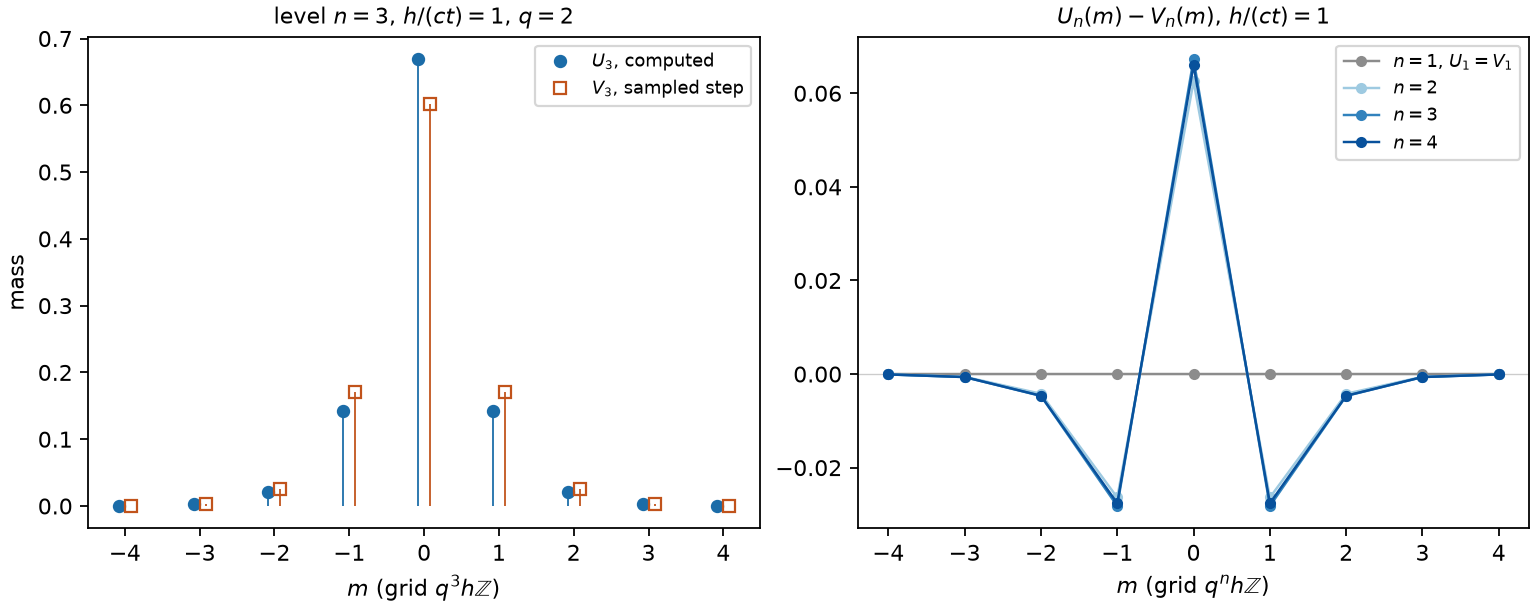
\includegraphics[width=\textwidth]{theory-grid-steps.png}
\caption{Proposition~\ref{prop:sampled-laplace-exact}(2) at $q = 2$ and $h/(ct) = 1$, in the units
of the grid $q^nh\ZZ$. Left: the computed array $U_3$, from $u_0 = \delta_0$ by three levels of
recursion and decimation, and the sampled step $V_3$, the samples of
$L_{ct} * L_{ctq} * L_{ctq^2}$ on $q^3h\ZZ$, both renormalized to unit mass. Right:
$U_n(m) - V_n(m)$ for $n = 1, \dots, 4$. At $n = 1$ the run gives at most $10^{-16}$, which is
rounding. From $n = 2$ on, the difference at the centre lies between $0.062$ and $0.068$. Half the
$\ell^1$ norm of the difference is the distance of Table~\ref{tab:grid-pyramid-error}.}
\label{fig:theory-grid-steps}
\end{figure}

The samples of the Gaussian kernel on a grid, the first family one would try there, do not form a
convolution semigroup [\sscite{lindeberg1990scalespace}, Prop.~12 and the remark after it, p.~242]. Renormalized, they need not
form a hemigroup either. The script \texttt{scripts/sampled\_gaussian\_increments.py} computes the
step between two renormalized sampled Gaussians, as the inverse transform of the ratio of their
discrete transfers, for four pairs of standard deviations in grid units. Each Gaussian is sampled
at the $4096$ sites $-2048, \dots, 2047$, renormalized there, and read on the periodic grid of those
sites. Between $0.5$ and $0.6$ the step's least coefficient is $-0.011$, and between $1.0$ and
$1.2$ it is $-0.0046$, both at the sites $\pm 2$. Between $2.0$ and $2.5$ the least coefficient is
$-2.8 \times 10^{-7}$, at $\pm 10$. Between $0.7$ and $3.0$ the double-precision value is rounding.
The script evaluates that pair again at $60$ digits, and the least coefficient is
$-2.8 \times 10^{-33}$, at $\pm 36$. These are computed signs on a periodic grid. Over the four
pairs the magnitude of the least coefficient falls as the larger standard deviation grows, and no inequality is proved here for
all scales.

For the first pair a short argument shows on the infinite lattice $\ZZ$ that no probability law
joins the two. Let $X$ and $Z$ have the sampled Gaussian laws of standard deviations $0.5$ and
$0.6$, normalized on $\ZZ$. Suppose $Z$ has the law of $X + Y$, with $Y$ a random variable
independent of $X$. Then $Y$ lives on $\ZZ$, since
$X$ has an atom at $0$. Its moments are finite, as those of $Z$ are, and $\mathbb{E}Y = 0$. The
second and fourth moments give
$\mathbb{E}Y^2 = \mathbb{E}Z^2 - \mathbb{E}X^2$ and
$\mathbb{E}Y^4 = \mathbb{E}Z^4 - \mathbb{E}X^4 - 6\,\mathbb{E}X^2\,\mathbb{E}Y^2$. The script
computes them, with the sums cut at $|k| \le 5$ and an omitted tail below $10^{-18}$:
$\mathbb{E}Y^2 = 0.1366$ and $\mathbb{E}Y^4 = 0.0160$. On the integers $Y^4 \ge Y^2$, so
$\mathbb{E}Y^4 \ge \mathbb{E}Y^2$, a contradiction. So no probability law joins the two sampled
Gaussians, and the sampled Gaussian family is not a hemigroup on $\ZZ$. The argument fails at the
other three pairs, where
$\mathbb{E}Y^4 \ge \mathbb{E}Y^2$.

What the Laplace samples have and the Gaussian samples lack is the factorization of
Proposition~\ref{prop:sampled-laplace-exact}(1). Every step of the sampled Laplace family is a
convolution of two one-sided geometric laws, each mixed with $\delta_0$ at the weight
$p \in [0,1)$. The factorization rests on the transfer (\ref{eq:sampled-laplace-transfer}), a
rational function of $e^{i\vartheta}$ with one pole inside and one outside the unit circle. That the
mixing weight is a probability, $p < 1$, needs $a_s < a_t$ as well. The samples of a Gaussian have
a theta function as their transfer instead.

The sampled Laplace mask is also infinitely divisible on the grid, so its grid pyramid is exact in
sense (iii), in the second stratum (Proposition~\ref{prop:grid-pyramids-infinitely-divisible}(4)).
So the grid offers two objects. One is an exact cascade, the sampled Laplace family. The other is a
pyramid covariant under $q$, the geometric pyramid of its mask. For an integer $q \ge 2$, the
\Matern{} pyramid computed on the grids computes the ladder increments of the geometric pyramid of
the mask $g = \lambda_{ct}$ of Proposition~\ref{prop:sampled-laplace-exact}(2)
(Proposition~\ref{prop:line-and-arrays}(2)). From its second level on, its arrays are not the
samples of the \Matern{} pyramid's steps (Proposition~\ref{prop:sampled-laplace-exact}(2)).

\paragraph{Relation to the continuum theory.} Two statements used in this section have continuum
counterparts in the cone module \progpaper{V-cone v0.1}. They are Lindeberg's generator, from the
supplement, and the criterion for masks.

\emph{The generator.} The Cin ray of step $\tau$ \prog{V-cone v0.1}{Lemma~3.1(1), p.~13}, the fully
covariant family with the exponent $\Cin(\tau\omega)$, has at the scale $t$ the generator
$t^{-1}\delta^2_{t\tau}$, one symmetric second difference (Theorem~\ref{thm:cited-A13}). Its step
grows with the scale. Lindeberg's generator (Proposition~\ref{prop:lindeberg-stratum-one}) is the
same second difference, held at the fixed step $h$.

\emph{The masks.} The continuum counterpart of
Proposition~\ref{prop:grid-pyramids-infinitely-divisible}(2)--(3) is Theorem~\ref{thm:cited-A20}.
For a symmetric infinitely divisible step with a rational transform, it gives the covariant interpolant by a
product formula and decides whether that interpolant is the exponent of a fully covariant family.
The \Matern{} pyramid of Theorem~\ref{thm:matern-pyramid} at $d = 1$ is its case
$R(\omega) = (1 + \omega^2)^{-1}$ read at the scale $ct$. Its octave step from $t$ to $qt$ is the
Laplace law of range $ct$. On the lattice the picture changes in the following ways.
\begin{enumerate}
\item Infinite divisibility must be checked. The binomial mask has a rational transfer in
$e^{i\vartheta}$ and is not infinitely divisible, and clause (1) of the proposition supplies the
check.
\item The profile, a density in the continuum, becomes the finite atomic measure $\varpi_w$, and the
interpolant's becomes $\sum_mT_{q^{-m}}\varpi_w$. This is the same series read on measures, so the
product formula survives. Its convergence, automatic for a rational $R$, becomes the logarithmic
moment of the mask, the condition that makes the series of dilates a \Levy{} measure.
\item The continuum's criterion for full covariance has no lattice counterpart, as the opening of
Section~\ref{subsec:grid-pyramids-line} noted. The folded \Levy{} measures of a fully covariant
family are absolutely continuous (Theorem~\ref{thm:lattice-line}(3)), so an atomic one belongs to
no such family. Clause (3) gives the lattice answer: no grid pyramid is exact in the third stratum.
\end{enumerate}
When its criterion holds, Theorem~\ref{thm:cited-A20} delivers a fully covariant interpolant. A
grid pyramid requires covariance under one ratio only. In place of the uniqueness of the interpolant it has the uniqueness of the
knot kernels. Between the knots a grid pyramid is undetermined, and no fully covariant member is
there to select. The supplement describes this freedom (Section~\ref{sec:line-surface}).
